\section{Results}
\label{sec:results}

We evaluate two outcomes of cross-granularity pretraining: the tissue information retained in each representation and the predictive relationships learned between representations. We first establish anatomical transfer to held-out sections, then examine how relational supervision enriches developmental information and organizes correspondence without making the granularities interchangeable. We finally test transformations at trained and unseen target granularities and use their predicted responses to characterize spatial context dependence.

\subsection{Frozen representations recover anatomy in held-out sections}
\label{sec:dual-view-identification}

Frozen ZoomST representations distinguish anatomical compartments on sections excluded from pretraining. We compare whole-section clustering with atlas annotations across all eight held-out MOSTA sections. Molecular features concatenate $e_8,e_{32},e_{128}$, spatial features concatenate $g_8,g_{32},g_{128}$, and joint features combine both views. All pretrained encoders remain frozen; the target-section readouts are specified in Appendix~\ref{app:dual-view}.

Joint ZoomST features achieve higher AMI than the evaluated public pretrained baselines on every held-out section, with an equal-section mean of 0.577, and remain competitive with target-fitted spatial methods (Table~\ref{tab:representation-summary}). The same features retain 52.7\% of physical 32-nearest neighbors on average, linking anatomical agreement to local spatial organization. The matched-update No Cross model has similar mean AMI (0.575), but lower neighbor retention (50.4\%). Thus, the full model retains anatomical discrimination while improving local spatial correspondence relative to this ablation.

\begin{table}[!htbp]
\centering\small
\caption{\textbf{Tissue mapping and neighbor retention on eight held-out MOSTA sections.} \textbf{(a)} AMI as mean $\pm$ sample SD over clustering seeds 42, 43, and 44; the summary averages sections equally within each seed. \textbf{(b)} Equal-section mean recovery of physical 32-nearest neighbors. Molecular and Spatial Views each concatenate three granularities; Joint combines both. No Cross uses the same joint readout and total training updates without cross-granularity supervision. Pretrained encoders are frozen. Bold marks the top three unrounded values per row, including third-place ties. Protocol: Appendix~\ref{app:dual-view}.}
\label{tab:representation-summary}
\label{tab:dual-view-sections}
\setlength{\tabcolsep}{0.8pt}
\renewcommand{\arraystretch}{1.05}
\begin{tabular}{lcccccccccc}
\toprule
 & \multicolumn{4}{c}{ZoomST Versions} & \multicolumn{2}{c}{Frozen pretrained} & \multicolumn{4}{c}{Target-fitted} \\
\cmidrule(lr){2-5}\cmidrule(lr){6-7}\cmidrule(lr){8-11}
Stage & Joint & \shortstack{Molecular\\View} & \shortstack{Spatial\\View} & \shortstack{No Cross\\Ablation} & Novae & SToFM & GraphST & BANKSY & MENDER & STAGATE \\
\midrule
\multicolumn{11}{l}{\textbf{(a) Anatomical agreement: AMI} $\uparrow$} \\
E9.5 & \textbf{0.547} & 0.486 & \textbf{0.556} & 0.533 & 0.371 & 0.211 & 0.538 & 0.540 & 0.530 & \textbf{0.556} \\
 & {\scriptsize $\pm 0.014$} & {\scriptsize $\pm 0.016$} & {\scriptsize $\pm 0.017$} & {\scriptsize $\pm 0.005$} & {\scriptsize $\pm 0.007$} & {\scriptsize $\pm 0.004$} & {\scriptsize $\pm 0.009$} & {\scriptsize $\pm 0.021$} & {\scriptsize $\pm 0.005$} & {\scriptsize $\pm 0.028$} \\
\addlinespace[2pt]
E10.5 & \textbf{0.549} & 0.516 & 0.534 & \textbf{0.549} & 0.390 & 0.262 & 0.534 & 0.539 & 0.531 & \textbf{0.544} \\
 & {\scriptsize $\pm 0.009$} & {\scriptsize $\pm 0.014$} & {\scriptsize $\pm 0.002$} & {\scriptsize $\pm 0.004$} & {\scriptsize $\pm 0.004$} & {\scriptsize $\pm 0.013$} & {\scriptsize $\pm 0.010$} & {\scriptsize $\pm 0.013$} & {\scriptsize $\pm 0.001$} & {\scriptsize $\pm 0.023$} \\
\addlinespace[2pt]
E11.5 & \textbf{0.628} & \textbf{0.608} & \textbf{0.615} & 0.602 & 0.444 & 0.291 & 0.502 & 0.573 & 0.561 & 0.559 \\
 & {\scriptsize $\pm 0.001$} & {\scriptsize $\pm 0.004$} & {\scriptsize $\pm 0.010$} & {\scriptsize $\pm 0.001$} & {\scriptsize $\pm 0.008$} & {\scriptsize $\pm 0.007$} & {\scriptsize $\pm 0.004$} & {\scriptsize $\pm 0.022$} & {\scriptsize $\pm 0.002$} & {\scriptsize $\pm 0.007$} \\
\addlinespace[2pt]
E12.5 & \textbf{0.613} & \textbf{0.614} & 0.607 & \textbf{0.618} & 0.447 & 0.307 & 0.509 & 0.583 & 0.582 & 0.585 \\
 & {\scriptsize $\pm 0.015$} & {\scriptsize $\pm 0.003$} & {\scriptsize $\pm 0.006$} & {\scriptsize $\pm 0.013$} & {\scriptsize $\pm 0.011$} & {\scriptsize $\pm 0.008$} & {\scriptsize $\pm 0.017$} & {\scriptsize $\pm 0.007$} & {\scriptsize $\pm 0.009$} & {\scriptsize $\pm 0.017$} \\
\addlinespace[2pt]
E13.5 & \textbf{0.578} & 0.541 & \textbf{0.579} & 0.573 & 0.432 & 0.334 & 0.386 & \textbf{0.593} & 0.573 & 0.544 \\
 & {\scriptsize $\pm 0.012$} & {\scriptsize $\pm 0.011$} & {\scriptsize $\pm 0.012$} & {\scriptsize $\pm 0.003$} & {\scriptsize $\pm 0.003$} & {\scriptsize $\pm 0.017$} & {\scriptsize $\pm 0.013$} & {\scriptsize $\pm 0.015$} & {\scriptsize $\pm 0.009$} & {\scriptsize $\pm 0.006$} \\
\addlinespace[2pt]
E14.5 & 0.563 & 0.556 & 0.558 & \textbf{0.571} & 0.450 & 0.407 & 0.453 & \textbf{0.572} & 0.535 & \textbf{0.579} \\
 & {\scriptsize $\pm 0.019$} & {\scriptsize $\pm 0.009$} & {\scriptsize $\pm 0.006$} & {\scriptsize $\pm 0.017$} & {\scriptsize $\pm 0.009$} & {\scriptsize $\pm 0.006$} & {\scriptsize $\pm 0.005$} & {\scriptsize $\pm 0.008$} & {\scriptsize $\pm 0.004$} & {\scriptsize $\pm 0.021$} \\
\addlinespace[2pt]
E15.5 & \textbf{0.626} & \textbf{0.625} & 0.614 & \textbf{0.630} & 0.494 & 0.405 & 0.422 & 0.614 & 0.600 & 0.604 \\
 & {\scriptsize $\pm 0.001$} & {\scriptsize $\pm 0.006$} & {\scriptsize $\pm 0.004$} & {\scriptsize $\pm 0.013$} & {\scriptsize $\pm 0.004$} & {\scriptsize $\pm 0.005$} & {\scriptsize $\pm 0.005$} & {\scriptsize $\pm 0.003$} & {\scriptsize $\pm 0.010$} & {\scriptsize $\pm 0.003$} \\
\addlinespace[2pt]
E16.5 & 0.513 & 0.497 & \textbf{0.532} & 0.524 & 0.449 & 0.331 & 0.403 & \textbf{0.526} & 0.509 & \textbf{0.540} \\
 & {\scriptsize $\pm 0.010$} & {\scriptsize $\pm 0.012$} & {\scriptsize $\pm 0.007$} & {\scriptsize $\pm 0.008$} & {\scriptsize $\pm 0.006$} & {\scriptsize $\pm 0.007$} & {\scriptsize $\pm 0.002$} & {\scriptsize $\pm 0.006$} & {\scriptsize $\pm 0.016$} & {\scriptsize $\pm 0.006$} \\
\addlinespace[2pt]
Mean AMI & \textbf{0.577} & 0.555 & \textbf{0.574} & \textbf{0.575} & 0.435 & 0.319 & 0.468 & 0.567 & 0.553 & 0.564 \\
 & {\scriptsize $\pm 0.004$} & {\scriptsize $\pm 0.006$} & {\scriptsize $\pm 0.003$} & {\scriptsize $\pm 0.003$} & {\scriptsize $\pm 0.001$} & {\scriptsize $\pm 0.003$} & {\scriptsize $\pm 0.003$} & {\scriptsize $\pm 0.003$} & {\scriptsize $\pm 0.002$} & {\scriptsize $\pm 0.0005$} \\
\addlinespace[2pt]
\midrule
\multicolumn{11}{l}{\textbf{(b) Local spatial organization} $\uparrow$} \\
\shortstack{Neighbor\\retention} & \textbf{0.527} & 0.502 & \textbf{0.523} & \textbf{0.504} & 0.313 & 0.033 & 0.268 & 0.483 & 0.354 & 0.354 \\
\bottomrule
\end{tabular}

\end{table}

The held-out E16.5 E2S13 Brain case illustrates the complementary information in the two views (Figure~\ref{fig:dual-view-brain}). Molecular features recover most Brain positions but include neighboring tissue; spatial features make fewer extra assignments but miss part of the Brain. Joint features reduce this tradeoff, increasing Brain IoU from 0.884 for $e$ and 0.905 for $g$ to 0.962. Whole-section maps and section-wise spatial retention are provided in Figures~\ref{fig:dual-view-e125} and~\ref{fig:dual-view-retention}. These results establish a transferable representation base from which to assess the additional value of learning granularity relationships.

\begin{figure}[!htbp]
\centering
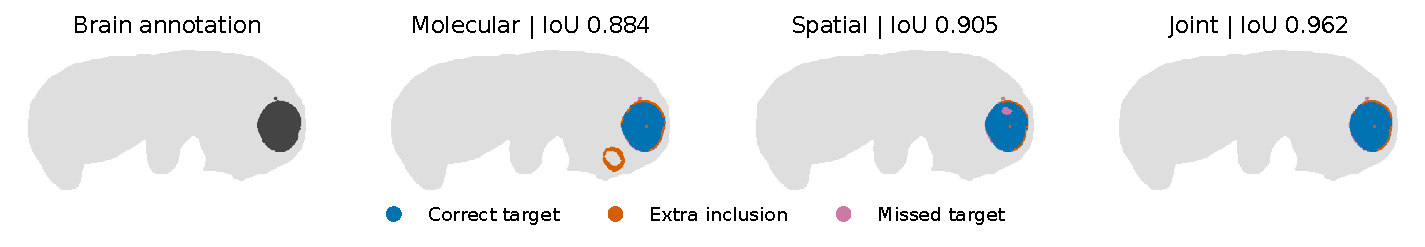
\includegraphics[width=\linewidth]{figures/brain_complementarity.pdf}
\caption{\textbf{Complementary molecular and spatial errors on a held-out section.} Annotation, molecular, spatial, and joint Brain assignments in E16.5 E2S13. Blue: correct assignments; orange: extra assignments; magenta: missed Brain. All maps use the same whole-section readout and seed 42. Each feature set combines its respective training granularities.}
\label{fig:dual-view-brain}
\end{figure}
\FloatBarrier

\subsection{Cross-granularity learning enriches developmental information}
\label{sec:developmental-information}

Having examined the two views in zero-shot tissue mapping, we next ask what cross-granularity learning adds to the retained representations. We compare the final ZoomST and No Cross checkpoints in an equal-budget controlled ablation. No Cross retains within-granularity learning and omits cross-granularity supervision. With both encoders frozen, we evaluate Joint separately at granularities 8, 32, and 128 on held-out MOSTA and HESTA sections, using independently pretrained mouse and human models (Appendix~\ref{app:preprocessing}).

Fine-granularity AMI improves on seven of eight held-out MOSTA sections and all seven HESTA sections (Table~\ref{tab:cross-granularity-ami}a). These AMI gains are modest, prompting us to ask whether the learned relations add information about developmental progression within the same tissue.


We examine Brain through two complementary tasks: developmental ordering and stage prediction. Diffusion pseudotime assesses agreement with the observed developmental sequence through spot-level Spearman correlation. A linear readout tests whether stage can be predicted from frozen representations, training on other sections and evaluating an entire held-out section. Together, these tasks measure unsupervised ordering and the stage information accessible to a supervised readout (Appendix~\ref{app:developmental-ordering}).

The developmental gains are particularly evident in coarse representations (Table~\ref{tab:cross-granularity-development}b). MOSTA shows its largest ordering improvement at the coarsest granularity, where spot-level correlation changes from negative to positive. HESTA shows higher spot-level correlations at every granularity. Stage-prediction error decreases at every granularity in both atlases, with the largest relative MAE reductions at $k=128$: 21.01\% on MOSTA and 8.73\% on HESTA. On MOSTA, adding JointMMD further reduces stage-prediction error relative to CS alone at all three granularities (Appendix~\ref{app:objective-ablation}). Cross-granularity learning thus enriches developmental information within broad tissue contexts, beyond its modest effect on anatomical clustering.

\begin{table}[!htbp]
\centering
\caption{\textbf{Cross-granularity learning across mouse and human atlases.} \textbf{(a)} Joint AMI, with SD over downstream clustering initializations below each mean; sections are averaged equally within each clustering run. Improved counts held-out sections with higher mean AMI. \textbf{(b)} Brain spot-level DPT correlation and leave-one-section-out stage MAE, in embryonic days for MOSTA and Carnegie stages for HESTA. Bold marks the better paired value, including ties. Evaluation protocols: Appendix~\ref{app:dual-view}--\ref{app:developmental-ordering}.}
\label{tab:cross-granularity-ami}
\label{tab:cross-granularity-development}
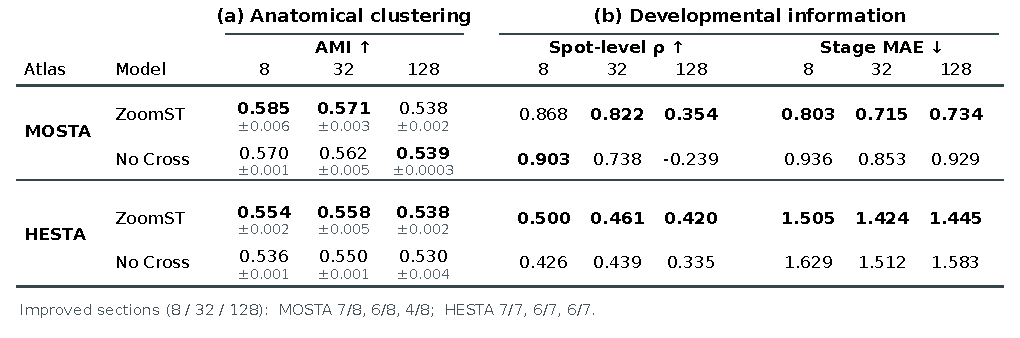
\includegraphics[width=\linewidth]{figures/cross_granularity_combined.pdf}
\end{table}
\FloatBarrier

This developmental information also gives ZoomST an advantage in cross-method comparisons (Figure~\ref{fig:developmental-ordering}). Combining all three granularities, ZoomST achieves the highest spot-level correlation on both MOSTA and HESTA among methods with complete-stage readouts. The ablation and cross-method results show that learning relations across granularities strengthens the developmental content of tissue representations while preserving their anatomical utility.

\begin{figure}[!htbp]
\centering
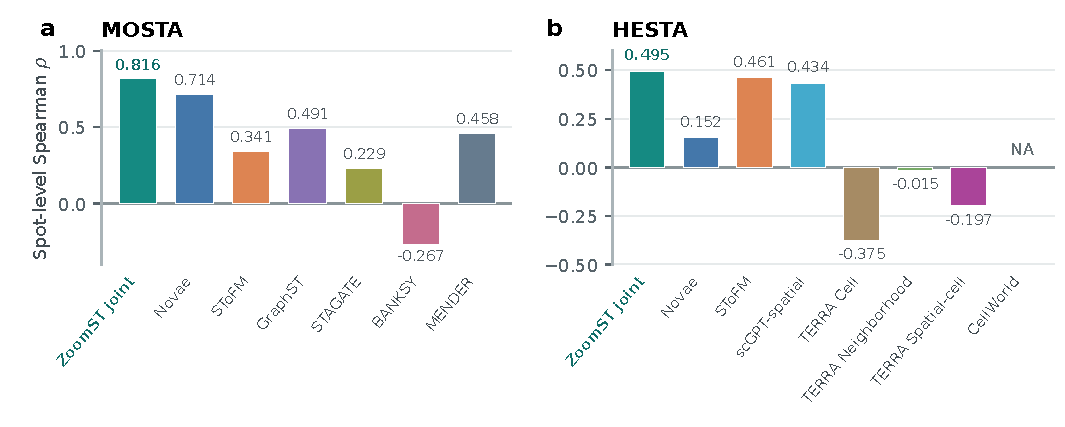
\includegraphics[width=0.98\linewidth]{figures/developmental_ordering_spearman.pdf}
\caption{\textbf{Developmental ordering on MOSTA and HESTA Brain.} Methods share observations and a fixed root within each atlas: (a) MOSTA, 4,712 spots; (b) HESTA, 2,560 spots. ZoomST combines Joint features from three granularities. NA: CellWorld does not connect CS18 to the root. Baseline fitting and DPT settings: Appendix~\ref{app:developmental-ordering}.}
\label{fig:developmental-ordering}
\end{figure}
\FloatBarrier

\subsection{Granularity-specific anatomical uses}
\label{sec:objective-ablation}

\label{sec:anatomical-scale-preference}
The retained granularities favor different anatomical regions. We compare ZoomST Spatial representations at granularities 8, 32, and 128 with six external methods across all 43 regions in the eight held-out sections. For each section, all methods share annotation-balanced clustering-fit positions and are scored on the full section by region-wise IoU (Appendix~\ref{app:region-scale}). Table~\ref{tab:regional-spatial-iou} highlights two patterns from the complete benchmark in Table~\ref{tab:regional-spatial-iou-full}. Locally homogeneous Spinal cord, Kidney, and Olfactory epithelium favor granularity 128, whereas boundary-rich Mucosal epithelium, Blood vessel, and Surface ectoderm favor granularity 8. Spinal cord IoU rises from 0.390 at granularity 8 to 0.489 at 128, while Blood vessel falls from 0.347 to 0.138. In these examples, the preferred ZoomST granularity also exceeds all six external methods. The choice of context therefore changes which anatomical structures the representation resolves best.

These scale preferences track the composition of the surrounding tissue. We measure neighborhood homogeneity by the mean same-label fraction among 128 spatial neighbors, and boundary fraction by the proportion of positions with at least one differently labeled neighbor among their eight nearest neighbors. Across 137 section--region observations, the coarse-scale gain, $\Delta\mathrm{IoU}=\mathrm{IoU}_{128}-\mathrm{IoU}_{8}$, increases with homogeneity and decreases with boundary fraction (Figure~\ref{fig:region-geometry}). The mean within-section Spearman correlations are 0.409 and $-0.337$, respectively, with each direction observed in seven of eight sections. Locally homogeneous structures therefore tend to benefit more from broad context, while regions with frequent boundaries favor finer context. The representations thus retain distinct anatomical uses after cross-granularity learning.

\begin{figure}[!htbp]
\centering
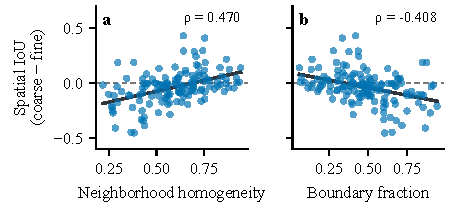
\includegraphics[width=\linewidth]{figures/region_geometry.pdf}
\caption{\textbf{Coarse-scale anatomical gains track neighborhood homogeneity and boundary frequency.} Each point is one of 137 section--region observations from eight held-out sections; colors and symbols identify developmental stages. The vertical axis is the Spatial IoU difference between granularities 128 and 8, in percentage points, after averaging three clustering seeds. Positive values favor coarse context. (a) Mean same-label fraction among 128 spatial neighbors. (b) Fraction of positions with a differently labeled neighbor among eight spatial neighbors. Geometry uses the full measured section, excluding each focal position from its own neighbor set. Solid lines show pooled linear fits; dashed lines mark equal IoU. The panels report pooled Spearman correlations and the mean of eight within-section correlations.}
\label{fig:region-geometry}
\end{figure}
\FloatBarrier
\begin{table}[!htbp]
\begingroup\centering\fontsize{8}{9}\selectfont
\setlength{\tabcolsep}{1.1pt}\renewcommand{\arraystretch}{1.02}
\caption{\textbf{Distinct anatomical structures favor coarse or fine Spatial context.} Selected examples from the complete 43-region benchmark in Table~\ref{tab:regional-spatial-iou-full}. The upper group favors granularity 128; the lower group favors granularity 8. In each example, the preferred ZoomST granularity also attains the highest IoU among the compared methods. Values are means with sample SD below across $n$ sections, after averaging three clustering seeds per section; single-section regions have one value. $H_{128}$ is neighborhood homogeneity. Bold marks the highest IoU across columns; underlining marks the best ZoomST granularity.}\label{tab:regional-spatial-iou}
\begin{tabular}{@{}>{\raggedright\arraybackslash}p{0.175\linewidth}cc*{9}{c}@{}}
\toprule
 & & & \multicolumn{3}{c}{ZoomST Spatial} & \multicolumn{2}{c}{Frozen pretrained} & \multicolumn{4}{c}{Target-fitted} \\
\cmidrule(lr){4-6}\cmidrule(lr){7-8}\cmidrule(l){9-12}
Region & $n$ & $H_{128}$ & 8 & 32 & 128 & Novae & SToFM & GraphST & BANKSY & MENDER & STAGATE \\
\midrule
\multicolumn{12}{l}{\textit{Coarse-context examples}}\\[3pt]
Spinal cord & 4 & 0.780 & \shortstack{0.390\\{\fontsize{7}{7.5}\selectfont $\pm0.108$}} & \shortstack{0.404\\{\fontsize{7}{7.5}\selectfont $\pm0.065$}} & \shortstack{\textbf{\underline{0.489}}\\{\fontsize{7}{7.5}\selectfont $\pm0.117$}} & \shortstack{0.311\\{\fontsize{7}{7.5}\selectfont $\pm0.172$}} & \shortstack{0.198\\{\fontsize{7}{7.5}\selectfont $\pm0.082$}} & \shortstack{0.436\\{\fontsize{7}{7.5}\selectfont $\pm0.166$}} & \shortstack{0.398\\{\fontsize{7}{7.5}\selectfont $\pm0.119$}} & \shortstack{0.402\\{\fontsize{7}{7.5}\selectfont $\pm0.089$}} & \shortstack{0.426\\{\fontsize{7}{7.5}\selectfont $\pm0.154$}} \\[2.2pt]
Kidney & 1 & 0.755 & 0.286 & 0.425 & \textbf{\underline{0.697}} & 0.045 & 0.136 & 0.639 & 0.007 & 0.007 & 0.112 \\[2.2pt]
Olfactory epithelium & 2 & 0.750 & \shortstack{0.540\\{\fontsize{7}{7.5}\selectfont $\pm0.372$}} & \shortstack{0.572\\{\fontsize{7}{7.5}\selectfont $\pm0.196$}} & \shortstack{\textbf{\underline{0.616}}\\{\fontsize{7}{7.5}\selectfont $\pm0.061$}} & \shortstack{0.412\\{\fontsize{7}{7.5}\selectfont $\pm0.027$}} & \shortstack{0.040\\{\fontsize{7}{7.5}\selectfont $\pm0.020$}} & \shortstack{0.528\\{\fontsize{7}{7.5}\selectfont $\pm0.301$}} & \shortstack{0.552\\{\fontsize{7}{7.5}\selectfont $\pm0.299$}} & \shortstack{0.463\\{\fontsize{7}{7.5}\selectfont $\pm0.433$}} & \shortstack{0.194\\{\fontsize{7}{7.5}\selectfont $\pm0.266$}} \\[2.2pt]
\midrule
\multicolumn{12}{l}{\textit{Fine-context examples}}\\[3pt]
Mucosal epithelium & 4 & 0.518 & \shortstack{\textbf{\underline{0.302}}\\{\fontsize{7}{7.5}\selectfont $\pm0.178$}} & \shortstack{0.260\\{\fontsize{7}{7.5}\selectfont $\pm0.112$}} & \shortstack{0.188\\{\fontsize{7}{7.5}\selectfont $\pm0.122$}} & \shortstack{0.221\\{\fontsize{7}{7.5}\selectfont $\pm0.174$}} & \shortstack{0.076\\{\fontsize{7}{7.5}\selectfont $\pm0.022$}} & \shortstack{0.270\\{\fontsize{7}{7.5}\selectfont $\pm0.189$}} & \shortstack{0.196\\{\fontsize{7}{7.5}\selectfont $\pm0.153$}} & \shortstack{0.212\\{\fontsize{7}{7.5}\selectfont $\pm0.160$}} & \shortstack{0.290\\{\fontsize{7}{7.5}\selectfont $\pm0.242$}} \\[2.2pt]
Blood vessel & 2 & 0.439 & \shortstack{\textbf{\underline{0.347}}\\{\fontsize{7}{7.5}\selectfont $\pm0.254$}} & \shortstack{0.306\\{\fontsize{7}{7.5}\selectfont $\pm0.110$}} & \shortstack{0.138\\{\fontsize{7}{7.5}\selectfont $\pm0.193$}} & \shortstack{0.127\\{\fontsize{7}{7.5}\selectfont $\pm0.039$}} & \shortstack{0.182\\{\fontsize{7}{7.5}\selectfont $\pm0.227$}} & \shortstack{0.001\\{\fontsize{7}{7.5}\selectfont $\pm0.001$}} & \shortstack{0.134\\{\fontsize{7}{7.5}\selectfont $\pm0.153$}} & \shortstack{0.218\\{\fontsize{7}{7.5}\selectfont $\pm0.231$}} & \shortstack{0.296\\{\fontsize{7}{7.5}\selectfont $\pm0.307$}} \\[2.2pt]
Surface ectoderm & 2 & 0.428 & \shortstack{\textbf{\underline{0.399}}\\{\fontsize{7}{7.5}\selectfont $\pm0.059$}} & \shortstack{0.304\\{\fontsize{7}{7.5}\selectfont $\pm0.063$}} & \shortstack{0.312\\{\fontsize{7}{7.5}\selectfont $\pm0.029$}} & \shortstack{0.154\\{\fontsize{7}{7.5}\selectfont $\pm0.054$}} & \shortstack{0.174\\{\fontsize{7}{7.5}\selectfont $\pm0.016$}} & \shortstack{0.256\\{\fontsize{7}{7.5}\selectfont $\pm0.133$}} & \shortstack{0.301\\{\fontsize{7}{7.5}\selectfont $\pm0.051$}} & \shortstack{0.226\\{\fontsize{7}{7.5}\selectfont $\pm0.157$}} & \shortstack{0.342\\{\fontsize{7}{7.5}\selectfont $\pm0.068$}} \\[2.2pt]
\bottomrule
\end{tabular}\par\endgroup
\end{table}


\FloatBarrier

\subsection{Learned transformations generalize to new sections and granularities}
\label{sec:granularity-transfer}
\label{sec:scale-continuum}

The preceding results concern directly encoded representations. We now ask whether the learned relationships themselves support prediction, first at trained target granularities on new sections and then at intermediate granularities absent from training. In both tests, a prediction uses only the source molecular state and the requested granularity. Direct encodings of the actual target neighborhoods provide the scoring references.

\paragraph{Trained relationships transfer to held-out sections.}
Across all eight held-out sections, transformed states have lower target MSE than unchanged fine states for each trained granularity pair (Figure~\ref{fig:generalization-summary}A). Equal-section mean reductions are 21.3\%, 27.0\%, and 11.8\% for $8\to32$, $8\to128$, and $32\to128$, respectively. Correct fine--predicted-coarse pairings also have lower joint-distribution discrepancy than shuffled pairings in every section and direction, including evaluation with projections unused in training (Figure~\ref{fig:generalization-summary}B). Shuffling preserves the predicted coarse marginal distribution but disrupts its association with the fine source. Together, the error reduction and pairing control support transferable, location-dependent fine--coarse relationships (Appendix~\ref{app:granularity-transfer}).

\paragraph{Discrete supervision supports unseen-granularity queries.}
With both encoder and transition frozen after training only at 8, 32, and 128, we query six unseen granularities---12, 16, 24, 48, 64, and 96---from the same $e_{i,8}$. Predictions reduce target MSE in all 48 held-out section--granularity conditions (Figure~\ref{fig:generalization-summary}A). Averaging prediction and unchanged-source errors over the six targets within each section, then averaging the section-level relative reductions, gives a 21.96\% reduction. Intermediate encodings are used only for evaluation. The same learned transformation can therefore predict descriptions at observation ranges beyond the discrete training set; all section-level errors and the separate PCA illustrations are provided in Appendix~\ref{app:unseen-state-detail}.

\begin{figure}[!htbp]
\centering
\begin{minipage}[t]{0.625\linewidth}
\centering\vspace{0pt}
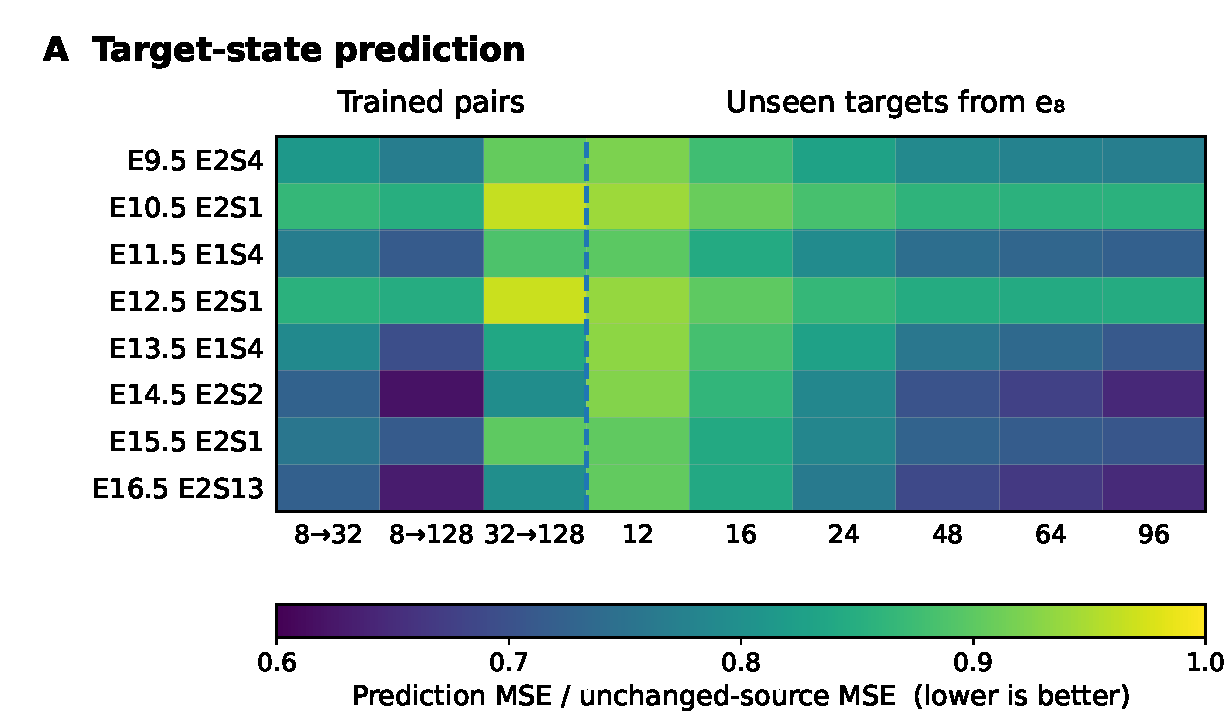
\includegraphics[width=\linewidth]{figures/results_generalization_matrix.pdf}
\end{minipage}\hfill
\begin{minipage}[t]{0.355\linewidth}
\centering\vspace{0pt}
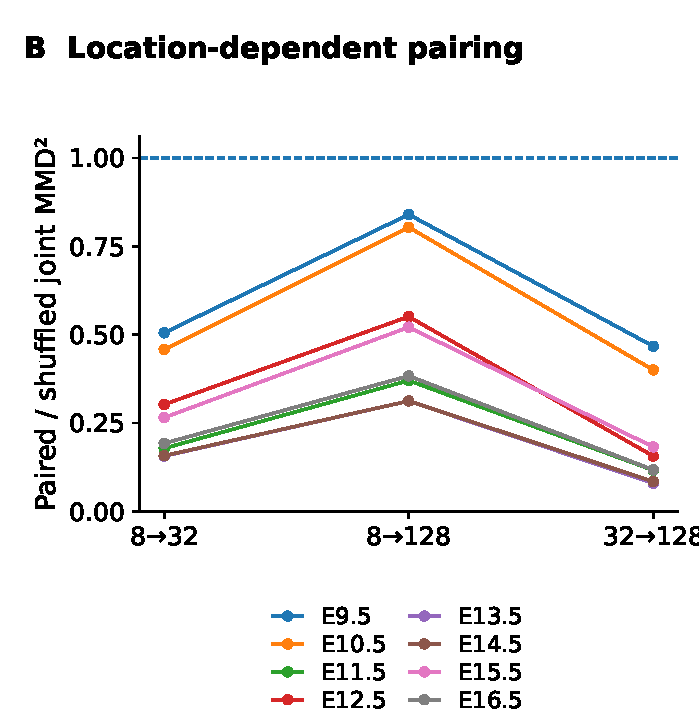
\includegraphics[width=\linewidth]{figures/results_pairing_control.pdf}
\end{minipage}
\caption{\textbf{Transformation generalization across held-out sections and observation granularities.} \textbf{A}, Target-MSE ratios for the three trained source--target pairs (left) and six unseen targets queried from $e_8$ (right). Each cell compares prediction with an unchanged source against the same directly encoded target. Trained-pair evaluation uses all section positions; unseen-target evaluation uses 1,024 fixed positions per section. All 24 trained-pair and 48 unseen-target ratios are below one. \textbf{B}, Correct-pair to shuffled-pair joint-MMD ratios for the trained pairs, averaged over four batches and eight projections unused in training. Each line is one held-out section. Values are from Tables~\ref{tab:granularity-transfer-sections} and~\ref{tab:ode-intermediate-sections}.}
\label{fig:generalization-summary}
\end{figure}

\paragraph{Continuous parameterization improves a matched prediction task.}
In a separate comparison on a shared frozen encoder, the neural ODE reduces mean unseen-granularity MSE by 10.86\% relative to a granularity-conditioned residual MLP, with lower error on all eight held-out sections. Both heads use the same source states and encoded targets (Appendix~\ref{app:transition-comparison}). This matched comparison supports the continuous parameterization; the preceding held-out tests establish the predictive capability of the jointly trained model.
\FloatBarrier

\subsection{Predicted responses reveal relative spatial context sensitivity}
\label{sec:context-response}

Once a transformation predicts states at different observation ranges, their differences can be used to compare context dependence across locations. We evaluate the normalized response in Equation~\ref{eq:granularity-response} against directly encoded changes over the same intervals, with all predictions starting from a common $e_8$.

\paragraph{Predicted response orders context-sensitive locations.}
For each held-out section and each of four doubling intervals, we rank 1,024 locations by predicted response and compare the highest and lowest quarters. The high-response quarter has a larger mean directly encoded change in 31 of 32 section--interval conditions (Figure~\ref{fig:heldout-response-ordering}). Equal-section mean high-to-low ratios range from 1.440 to 1.673 across the four intervals. Predicted response thus identifies relative differences in how strongly tissue descriptions depend on observation range (Appendix~\ref{app:response-meaning}).

\begin{figure}[!htbp]
\centering
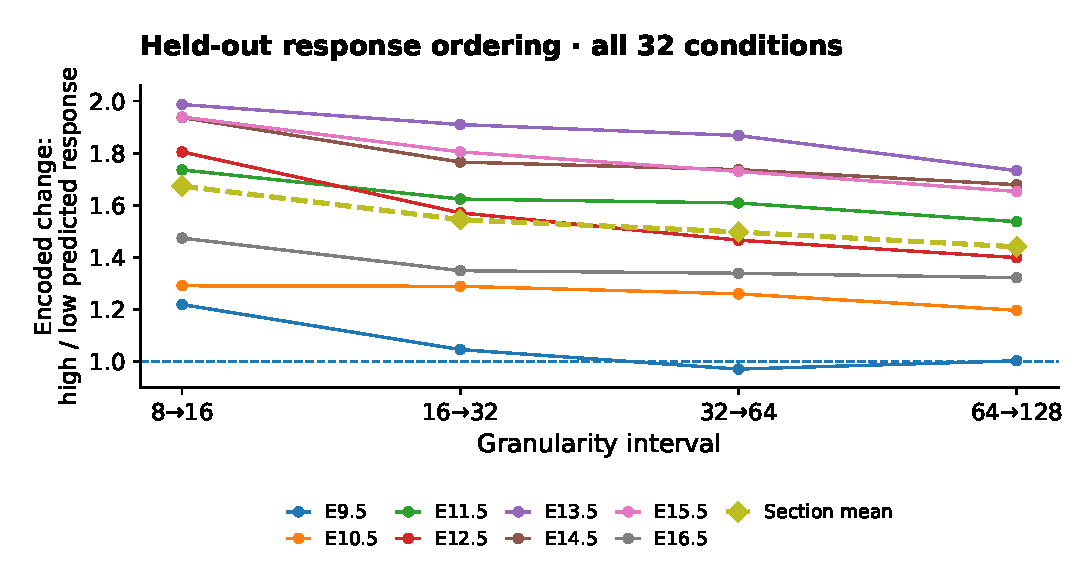
\includegraphics[width=0.78\linewidth]{figures/results_response_ordering.pdf}
\caption{\textbf{Predicted response identifies larger encoded changes on held-out sections.} Locations are ranked separately within each section and interval by predicted finite response. The ordinate is the ratio of mean directly encoded change in the highest versus lowest predicted-response quarter, with 256 locations per group. All 32 section--interval conditions are shown; 31 are above one. Lines denote sections and diamonds denote equal-section means. Full values: Table~\ref{tab:ode-response-heldout}.}
\label{fig:heldout-response-ordering}
\end{figure}

\paragraph{Anatomical context gives the response an interpretation.}
Two source-section cases illustrate distinct forms of context dependence. In E14.5 E1S1 Facial nerve, predicted and directly encoded changes correlate over $64\to128$ across all 64 locations ($\rho=0.791$; Figure~\ref{fig:scale-continuum}C). Predicted response also correlates with changes in annotated neighbor composition ($\rho=0.707$; Figure~\ref{fig:ode-context}A). In the highest-response quarter, the mean nerve fraction falls from 71.4\% to 45.7\% as context expands, compared with 43.4\% to 36.2\% in the lowest quarter (Figure~\ref{fig:ode-context}B). High-response locations therefore undergo a larger transition from a nerve-dominated neighborhood to surrounding tissue; low-response locations already include substantial surrounding tissue at the smaller range.

In E16.5 E1S1 Brain, context can change even when a broad annotation does not. Over $8\to16$, 95 sampled locations have only Brain-labeled neighbors at both granularities, yet their predicted and directly encoded responses correlate at $\rho=0.645$ (Appendix~\ref{app:response-meaning}). The response therefore captures molecular-context variation within a broad anatomical label as well as shifts in tissue composition. Whole-section maps illustrate the spatial heterogeneity of this dependence (Figure~\ref{fig:ode-context}C,D).

\begin{figure}[H]
\centering
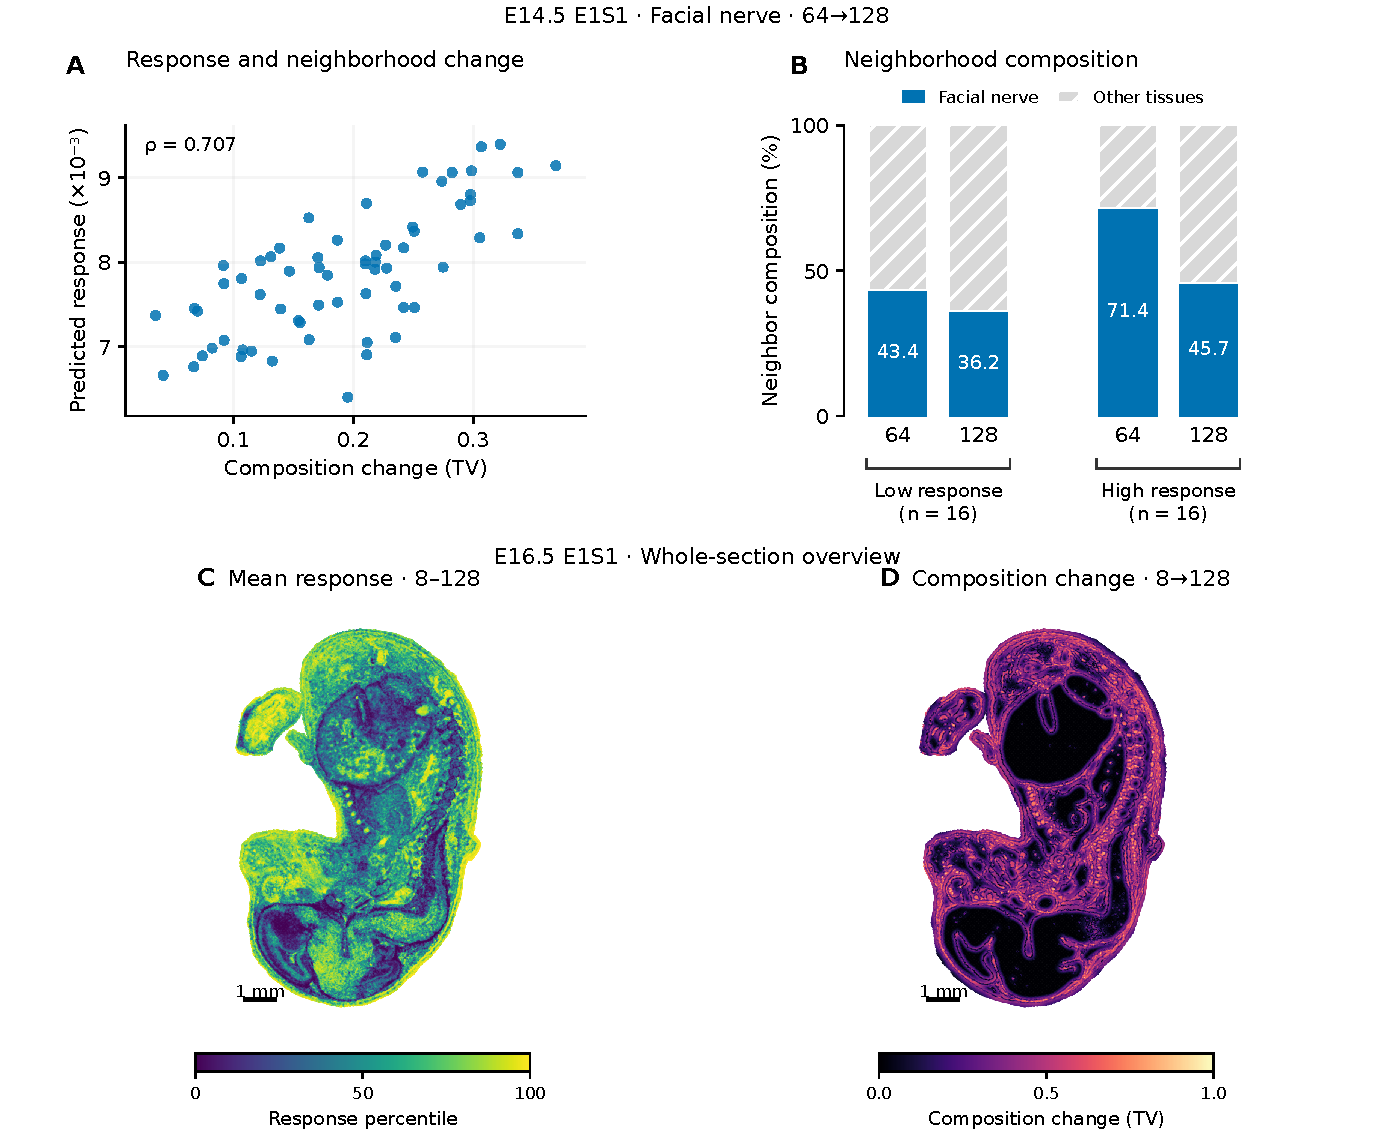
\includegraphics[width=0.92\linewidth]{figures/response_and_neighborhood_context.pdf}
\caption{\textbf{Context response distinguishes different dependencies on surrounding tissue.} \textbf{A}, Predicted finite response versus annotation-composition change (total variation, TV) at all 64 E14.5 E1S1 Facial nerve locations over $64\to128$. \textbf{B}, Mean composition at 64 and 128 for the lowest and highest response quarters, following the same 16 locations per group. \textbf{C,D}, E16.5 E1S1 whole-section maps of path-averaged instantaneous response over 8--128 (percentiles) and observed composition change from 8 to 128. These are spatial overviews of different quantities. All 121,767 locations are retained without smoothing. Both sections are anatomical cases from the training set; predictions start from fixed $e_8$. Scale bars: 1\,mm. Definitions: Appendix~\ref{app:response-meaning}.}
\label{fig:ode-context}
\end{figure}

\FloatBarrier
